\documentclass{beamer} \usetheme{Madrid}
\usecolortheme{beaver}

\usepackage[utf8]{inputenc}
\usepackage{mdframed}
\usepackage{mathtools}
\usepackage{minted}
\usepackage{siunitx}

\title{Arduino: Anatomy of a Blink}

\author{Jack Leightcap}

\institute[Wireless Club]{
    \url{neuwireless.slack.com}
    \and
    \url{leightcap.j@northeastern.edu}
}

\date[Fall 2020]{November 5, 2020}

\begin{document}
\definecolor{bg}{rgb}{0.95,0.95,0.95} % minted backgrounds
\frame{\titlepage}

\begin{frame}
    \frametitle{Outline}
    \begin{columns}[t]
        \begin{column}{{\textwidth}/2}
            \begin{center}
                \textbf{Languages}
            \end{center}
            \begin{itemize}
                \item Arduino IDE
                \item Bare C
                \item AVR Assembly
                \item Rust (new \& fancy)
                \item Building steps for each language
            \end{itemize}
        \end{column}
        \begin{column}{{\textwidth}/2}
            \begin{center}
                \textbf{Topics Along the Way}
            \end{center}
            \begin{itemize}
                \item Boolean Logic
                \item Systems Software
                \item Computer Architecture
                \item Comparison and Classifications of Programming Languages
            \end{itemize}
        \end{column}
    \end{columns}
\end{frame}

\begin{frame}[fragile]
    \frametitle{Arduino IDE: Blink}
    \begin{figure}
        \begin{minted}[
            fontsize=\scriptsize,
            numbersep=1pt,
            frame=lines,
            bgcolor=bg,
            framesep=3mm
        ]{C}
void setup() {
    pinMode(LED_BUILTIN, OUTPUT);
}

void loop() {
    digitalWrite(LED_BUILTIN, HIGH);
    delay(1000);
    digitalWrite(LED_BUILTIN, LOW);
    delay(1000);
}
        \end{minted}
        \caption{\texttt{blink.ino}}
    \end{figure}
\end{frame}

\begin{frame}
    \frametitle{Arduino IDE: Analysis}
    \vfill
    \textbf{Arduino Language}
    \begin{itemize}
        \item Not \emph{really} a programming language per se?
        \item Subset of C++ with Arduino-specific libraries/defaults
        \item Provides \texttt{pinMode()}, \texttt{LED\_BUILTIN}, \texttt{HIGH}, etc.
    \end{itemize}
    \vfill
    \textbf{Running}
    \begin{itemize}
        \item Just press ``Verify'' and ``Upload''
        \item Hides most build steps unless error
        \item Full output: \texttt{File $\rightarrow$ Preferences $\rightarrow$ verbose output}
    \end{itemize}
    \vfill
\end{frame}

\begin{frame}
    \frametitle{Masks: Setting/Resetting Bits}
    \vfill
    \begin{center} \textbf{Masking Bits to 1:} \end{center}
    \begin{itemize}
        \item $Y + 1 = 1$ and $Y + 0 = Y$ \hfill ($+$ is bitwise OR)
        \item
            \begin{tabular}{cc|c}
                $x$ & mask $m$ & $x + m$ \\
                \hline
                $00001001$ & $10000001$ & $10001001$ \\
            \end{tabular}
        \item \texttt{x = x | 0b10000001} $\rightarrow$ \texttt{x |= 0b10000001}
    \end{itemize}
    \vfill
    \begin{center} \textbf{Masking Bits to 0:} \end{center}
    \begin{itemize}
        \item $Y * 0 = 0$ and $Y * 1 = Y$ \hfill ($*$ is bitwise AND)
        \item
            \begin{tabular}{cc|c}
                $x$ & mask $m$ & $x * m$ \\
                \hline
                $00001001$ & $01111110$ & $00001000$ \\
            \end{tabular}
        \item \texttt{x = x \& 0b01111110} $\rightarrow$ \texttt{x \&= 0b01111110} $\rightarrow$ \texttt{x \&= \textasciitilde0b10000001}
    \end{itemize}
    \vfill
\end{frame}

\begin{frame}
    \frametitle{Arduino Port Registers}
    \textbf{Data Direction Registers}, \texttt{DDR*}
    \begin{itemize}
        \item $0$ at position $i$ indicates pin $i$ is read only
        \item $1$ at position $i$ indicates pin $i$ is write only
    \end{itemize}
    \textbf{Data Registers}, \texttt{PORT*}
    \begin{itemize}
        \item writing to read only undefined, reading from write only undefined
    \end{itemize}
    \begin{columns}[t]
        \begin{column}{{\textwidth}/3}
            \begin{center}\textbf{PORT B}\end{center}
            \begin{itemize}
                \item digital pins 8-15
                \item last two pins map to clock
            \end{itemize}
        \end{column}
        \begin{column}{{\textwidth}/3}
            \begin{center}\textbf{PORT C}\end{center}
            \begin{itemize}
                \item analog pins
                \item ADCs
            \end{itemize}
        \end{column}
        \begin{column}{{\textwidth}/3}
            \begin{center}\textbf{PORT D}\end{center}
            \begin{itemize}
                \item digital pins 0-7
                \item first two pins serial communication
            \end{itemize}
        \end{column}
    \end{columns}
\end{frame}

\begin{frame}
    \vfill
    \begin{center}
    \begin{figure}
        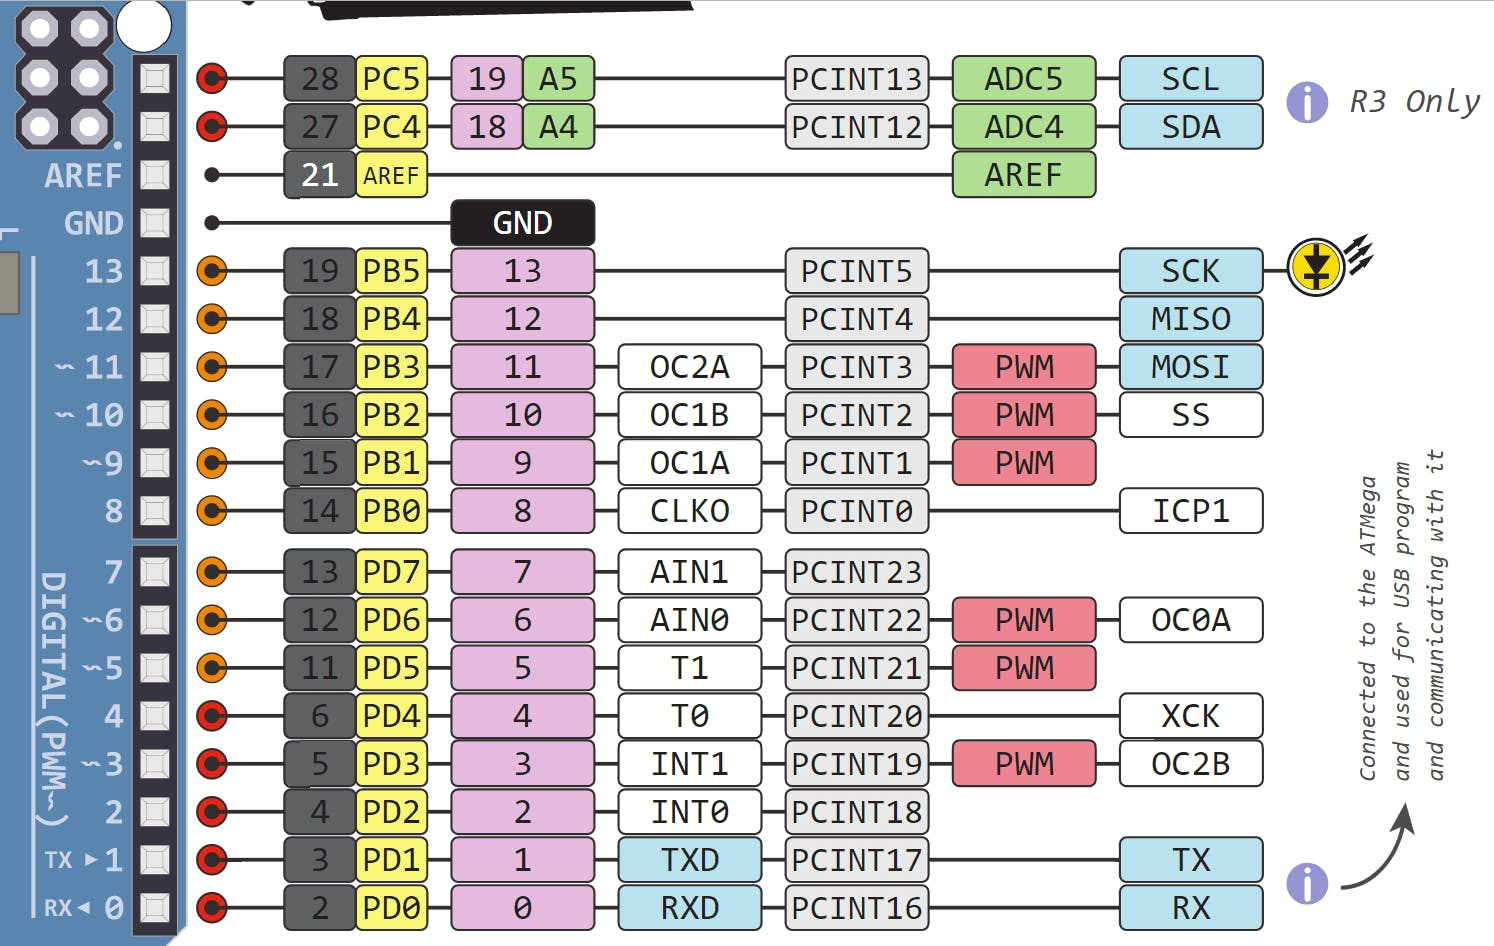
\includegraphics[width=4in]{arduinopins.png}
        \caption{\href{https://www.circuito.io/blog/arduino-uno-pinout/}{Arduino Uno Digital Pins, CC BY-SA}}
    \end{figure}
    \end{center}
    \vfill
\end{frame}

\begin{frame}[fragile]
    \frametitle{C: Blink}
    \begin{figure}
        \begin{minted}[
            fontsize=\scriptsize,
            numbersep=1pt,
            frame=lines,
            bgcolor=bg,
            framesep=3mm
        ]{C}
int
main(void)
{
    DDRB |= _BV(DDB5);
    while(1) {
        PORTB |= _BV(PORTB5);
        _delay_ms(1000);
        PORTB &= ~_BV(PORTB5);
        _delay_ms(1000);
    }
    return 0;
}
        \end{minted}
        \caption{\texttt{blink.c}}
    \end{figure}
\end{frame}

\begin{frame}
    \frametitle{Systems Software: \emph{Compiler}}
    \vfill
    \begin{itemize}
        \item Transform the text of one programming language into another
            \begin{center}
                Source Language $\xrightarrow{compiler}$ Target Language
            \end{center}
        \item \emph{Compiler} usually implies transforming into a lower level language
        \item \emph{Decompiler} transforms language into something of higher level
        \item \emph{Transpiler} transforms language into something of the same level
    \end{itemize}
    \vfill
    For the Arduino specifically, we'll be using two compilers:
    \begin{itemize}
        \item C to Arduino: \texttt{avr-gcc}
        \item Rust to Arduino: \texttt{LLVM} through \texttt{rustc}
        \item Target language is \href{https://en.wikipedia.org/wiki/Intel_HEX}{Intel HEX} formatted for the Arduino CPU
    \end{itemize}
    \vfill
\end{frame}

\begin{frame}[fragile]
    \frametitle{C: Compiling and Deploying}
    \vfill
    \begin{figure}
        \begin{minted}[
            fontsize=\scriptsize,
            numbersep=1pt,
            frame=lines,
            bgcolor=bg,
            framesep=3mm
        ]{bash}
# C -> ELF
$ avr-gcc -Os -DF_CPU=16000000UL -mmcu=atmega328p -o blink blink.c
# ELF -> HEX
$ avr-objcopy -O ihex -R .eeprom blink blink.hex
        \end{minted}
        \caption{C $\xrightarrow{\texttt{avr-\{gcc,objcopy\}}}$ Intel HEX}
    \end{figure}
    \vfill
    \begin{figure}
        \begin{minted}[
            fontsize=\scriptsize,
            numbersep=1pt,
            frame=lines,
            bgcolor=bg,
            framesep=3mm
        ]{bash}
# HEX -> Arduino
$ avrdude -F -V -c arduino -p ATMEGA328P -P /dev/ttyACM0 -b 115200 \
          -U flash:w:blink.hex
        \end{minted}
        \caption{Intel HEX $\xrightarrow{\texttt{avrdude}}$ Arduino}
    \end{figure}
    \vfill
\end{frame}

\begin{frame}
    \frametitle{Quick Intro to Assembly}
    \vfill
    \textbf{Assembly `Language'}
    \begin{itemize}
        \item Not a programming language, but a family of languages
        \item CPU and Architecture specific!
        \item AVR Assembly, ARM Assembly, x86\_64 Assembly, etc.
        \item Direct mapping to CPU instructions
        \item Oldest family of languages
    \end{itemize}
    \vfill
    \textbf{Arduino Uno CPU and Architecture}
    \begin{itemize}
        \item ATmega328P AVR microcontroller
        \item 8-bit RISC Instruction Set Architecture (ISA)
        \item 16MHz clock speed
        \item Harvard Architecture
        \item 32KB Flash memory store instructions/data, 2KB SRAM store data
    \end{itemize}
    \vfill
\end{frame}

\begin{frame}
    \vfill
    \begin{center} \begin{figure}
        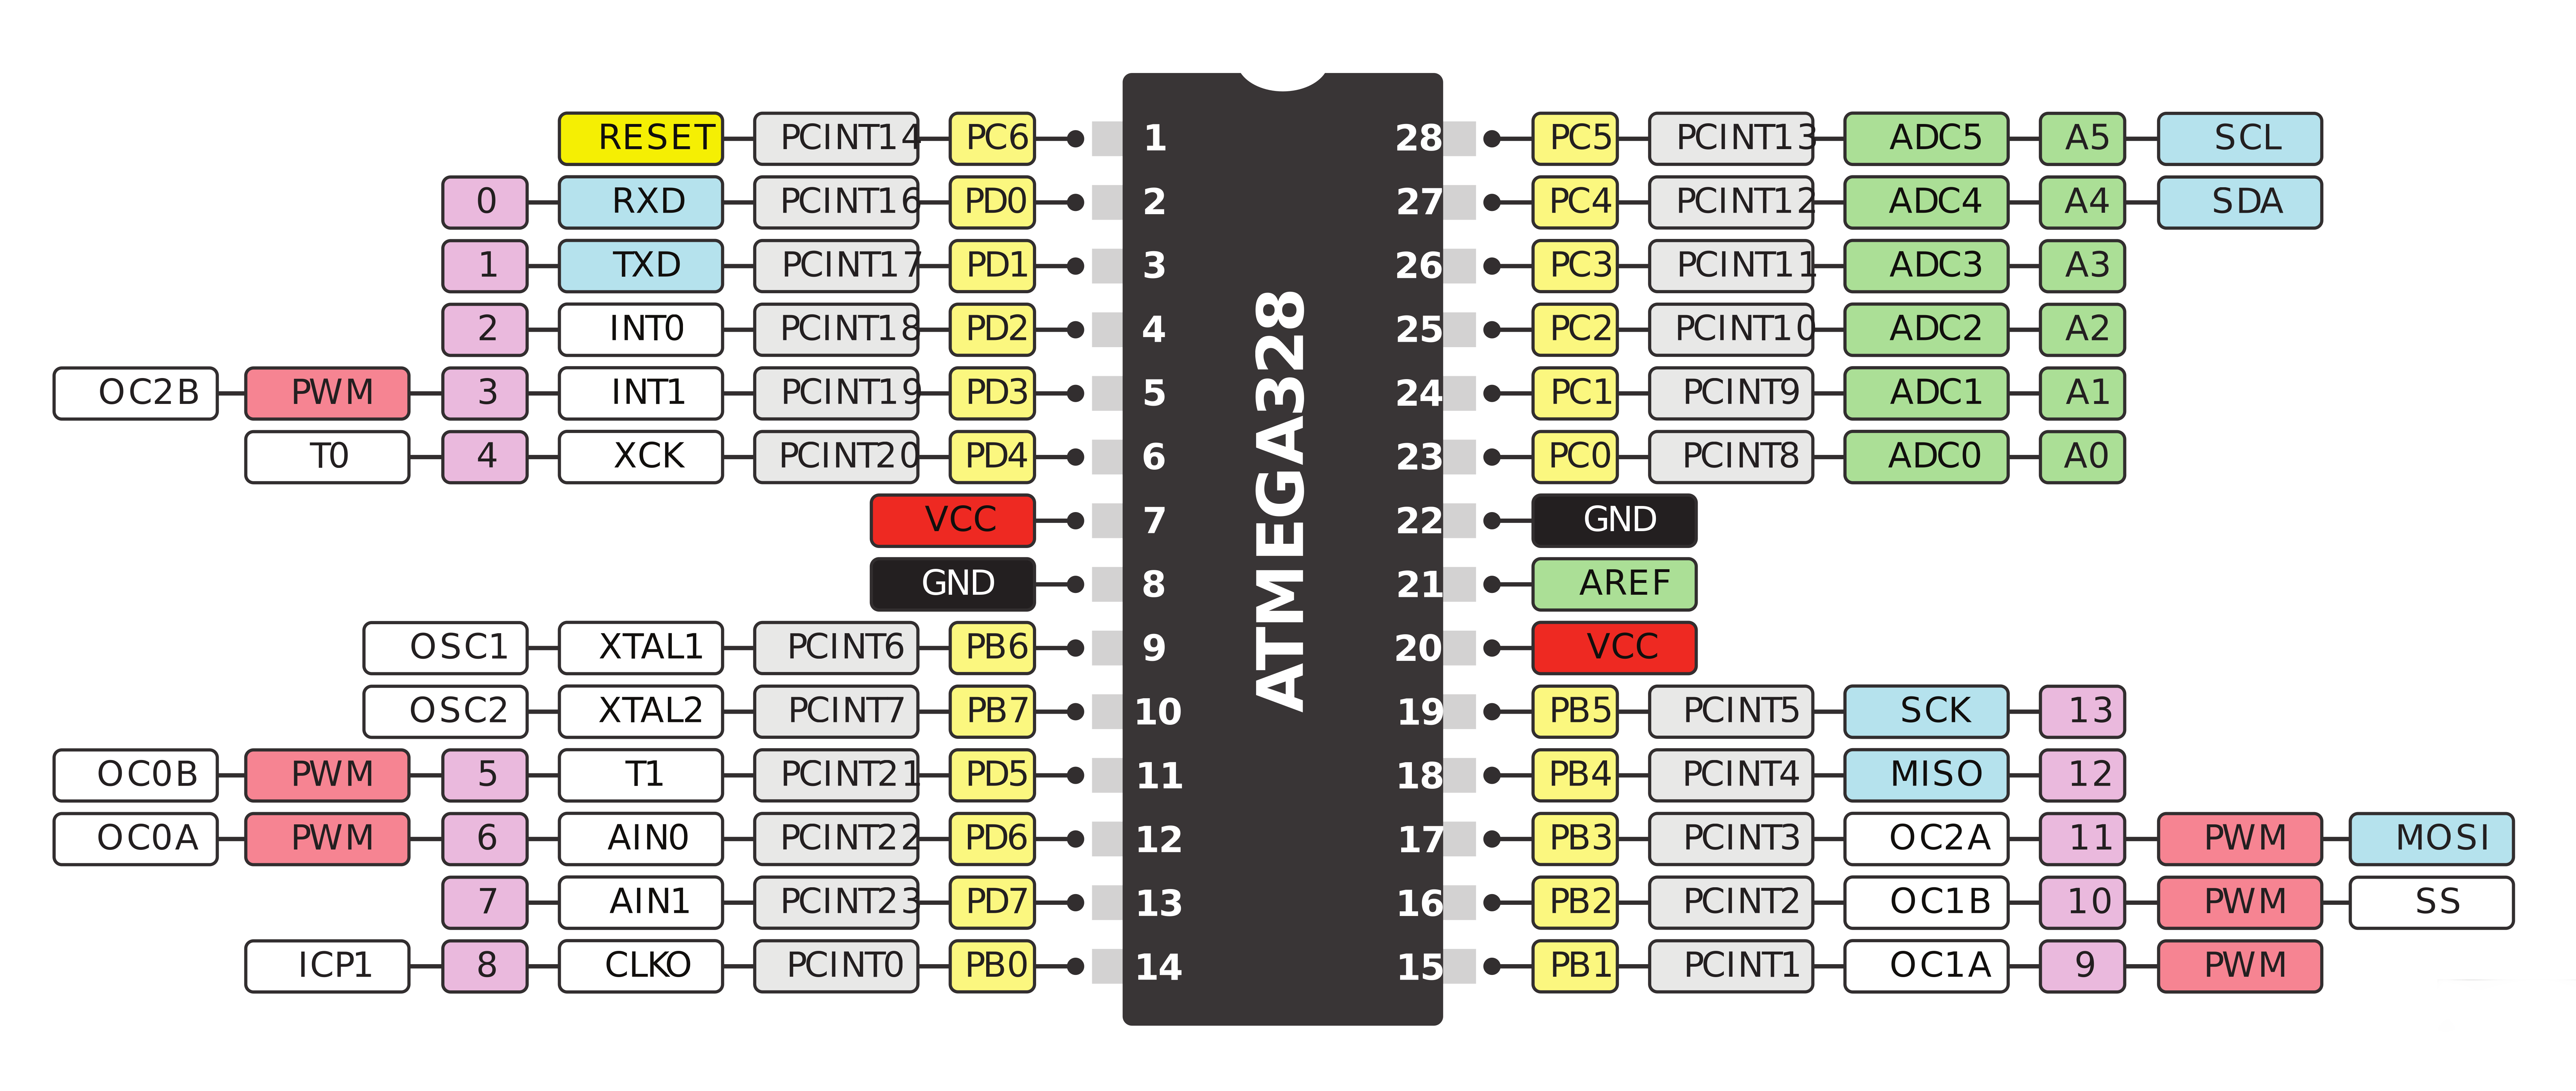
\includegraphics[width=\textwidth]{atmega_pinout.png}
        \caption{\href{https://commons.wikimedia.org/wiki/File:Pinout_of_ARDUINO_Board_and_ATMega328PU.svg}{ATmega328P Pinout, CC BY-SA}}
    \end{figure} \end{center}
    \vfill
\end{frame}

\begin{frame}
    \frametitle{Timings in Assembly}
    \begin{itemize}
        \item How many clock cycles in \(1\si{s}\)?
        \[
            \underbrace{1\si{s}}_{\text{time}}
            \times
            \underbrace{\frac{16*10^6 \text{cycles}}{1\si{s}}}_{\text{clock speed}}
            =
            16*10^6 \text{cycles}
        \]
        \item How many instructions is $16*10^6$ cycles?
        \item AVR is a RISC: instructions take exactly one cycle
        \item Use 3 registers (8-bits),
        \[
            16*10^6\text{cycles} \approx 256\text{cycles} \times 256\text{cycles} \times 244\text{cycles}
        \]
    \item Overflow two registers ($255 \rightarrow 0$), count down from $244$ in another
    \end{itemize}
\end{frame}

\begin{frame}[fragile]
    \frametitle{AVR Assembly: Blink}
    \begin{figure}
    \begin{columns}[t]
        \begin{column}{{\textwidth}/2}
            \begin{minted}[
                fontsize=\scriptsize,
                numbersep=1pt,
                frame=lines,
                bgcolor=bg,
                framesep=3mm
            ]{nasm}
.equ DDRB, 0x04
.equ PORTB, 0x05
.org 0x0000
rjmp RESET
RESET:
    ldi R16, 0x20
    out DDRB, R16
    ldi R18, 0x00
    ldi R17, 0x00
    ldi R20, 0x20
; cont...
            \end{minted}
        \end{column}
        \begin{column}{{\textwidth}/2}
            \begin{minted}[
                fontsize=\scriptsize,
                numbersep=1pt,
                frame=lines,
                bgcolor=bg,
                framesep=3mm
            ]{nasm}
Loop:
    ldi R19, 0xF4
delay:
    inc R17
    cpi R17, 0x00
    brne delay
    inc R18
    cpi R18, 0x00
    brne delay
    inc R19
    cpi R19, 0x00
    brne delay
    eor R16, R20
    out PORTB, R16
    rjmp Loop
            \end{minted}
        \end{column}
    \end{columns}
    \caption{\texttt{blink.asm}}
    \end{figure}
\end{frame}

\begin{frame}
    \frametitle{Systems Software: \emph{Assembler}}
    \vfill
    \begin{itemize}
        \item Tranform Assembly into machine code
            \begin{center}
                Assembly $\xrightarrow{assembler}$ Machine Code
            \end{center}
        \item Maybe a type of compiler, is machine code a language?
        \item Some optimizations (jump length)
        \item Definitions: variable names (\texttt{DDRB}, \texttt{PORTB}), locations (\texttt{RESET}, \texttt{delay})
        \item Directives: specify location with \texttt{.org 0x0000}
        \item Compiler calls Assembler in background
    \end{itemize}
    \vfill
    For the Arduino specifically:
    \begin{itemize}
        \item \texttt{avr-as}, what \texttt{avr-gcc} calls in the background
        \item Rust targeting AVR still requires \texttt{avr-as}, but choice of assembler for other architectures
    \end{itemize}
    \vfill
\end{frame}

\begin{frame}[fragile]
    \frametitle{AVR Assembly: Assembling and Deploying}
    \begin{figure}
        \begin{minted}[
            fontsize=\scriptsize,
            numbersep=1pt,
            frame=lines,
            bgcolor=bg,
            framesep=3mm
        ]{bash}
# AVR Assembly -> Object file
$ avr-as blink.asm -o blink.o
# Object file -> ELF
$ avr-ld -Ttext 0 -nostdlib -nostartfiles  blink.o -o blink.elf
# ELF -> HEX
$ avr-objcopy -O ihex blink.elf blink.hex
        \end{minted}
        \caption{AVR Assembly $\xrightarrow{\texttt{avr-\{as,ld,objcopy\}}}$ Intel HEX}
    \end{figure}
    \begin{figure}
        \begin{minted}[
            fontsize=\scriptsize,
            numbersep=1pt,
            frame=lines,
            bgcolor=bg,
            framesep=3mm
        ]{bash}
# HEX -> Arduino
$ avrdude -F -V -c arduino -p ATMEGA328P -P /dev/ttyACM0 -b 115200 \
          -U flash:w:blink.hex
        \end{minted}
        \caption{Intel HEX $\xrightarrow{\texttt{avrdude}}$ Arduino}
    \end{figure}
\end{frame}


\begin{frame}
    \frametitle{Quick Intro to Rust}
    \vfill
    \begin{center}
        \begin{tabular}{l|l}
            \textbf{Language} & \textbf{First Appeared}\\
            \hline
            Assembly & Ada Lovelace (1843), Kathleen Booth (1947) Atmel (1996) \\
            C & Dennis Ritchie and Ken Thompson (1972) \\
            C++ & Bjarne Stroustrup (1985) Arduino (2005) \\
            Rust & Graydon Hoare (2010)
       \end{tabular}
    \end{center}
    \vfill
    \begin{itemize}
        \item Very new (comparatively)
        \item Lots of benefits a small example won't show
        \item Memory safety, concurrency, high-level abstraction facilities
        \item ``Most loved programming language'' every year since 2016, Stack Overflow Developer Survey
    \end{itemize}
    \vfill
\end{frame}

\begin{frame}[fragile]
    \frametitle{Rust: Blink}
    \begin{figure}
    \begin{minted}[
        fontsize=\scriptsize,
        numbersep=1pt,
        frame=lines,
        bgcolor=bg,
        framesep=3mm
    ]{rust}
#![feature(llvm_asm)]
#![no_std]
#![no_main]
use ruduino::cores::atmega328 as avr_core;
use ruduino::Register;
use avr_core::{DDRB, PORTB};
fn small_delay() {
    for _ in 0..400000 { unsafe{llvm_asm!("" :::: "volatile")} }
}
#[no_mangle]
pub extern fn main() {
    DDRB::set_mask_raw(0xFFu8);
    loop {
        PORTB::set_mask_raw(0xFF);   small_delay();
        PORTB::unset_mask_raw(0xFF); small_delay();
    }
}
    \end{minted}
    \caption{\texttt{blink.rs}}
    \end{figure}
\end{frame}

\begin{frame}[fragile]
    \frametitle{Systems Software: \emph{Build Systems}}
    \begin{itemize}
        \item Saw the guts of how ``Verify'' and ``Upload'' work
        \item As complexity increases, building software becomes its own task
        \item Rust provides \texttt{cargo}
        \item \texttt{Makefile} common for C, \texttt{CMake} for C++; not provided by language
        \item Dependency management, build steps
    \end{itemize}
    \begin{figure}
    \begin{minted}[
        fontsize=\scriptsize,
        numbersep=1pt,
        frame=lines,
        bgcolor=bg,
        framesep=3mm
    ]{toml}
[package]
name = "blink"
version = "0.1.0"
authors = ["Dylan McKay <me@dylanmckay.io>"]
edition = '2018'
[dependencies]
ruduino = "0.2"
[profile.dev]
panic = "abort"
    \end{minted}
    \caption{\texttt{Cargo.toml} for \texttt{blink.rs}}
    \end{figure}
\end{frame}

\begin{frame}[fragile]
    \frametitle{Rust: Building and Deploying}
    \begin{figure}
        \begin{minted}[
            fontsize=\scriptsize,
            numbersep=1pt,
            frame=lines,
            bgcolor=bg,
            framesep=3mm
        ]{bash}
# Rust -> ELF
$ cargo build -Z build-std=core --target avr-atmega328p.json
        \end{minted}
        \caption{AVR Assembly $\xrightarrow{\texttt{avr-\{as,ld,objcopy\}}}$ Intel HEX}
    \end{figure}
    \begin{figure}
        \begin{minted}[
            fontsize=\scriptsize,
            numbersep=1pt,
            frame=lines,
            bgcolor=bg,
            framesep=3mm
        ]{bash}
# ELF -> Arduino
$ avrdude -D -F -V -c arduino -p ATMEGA328P -P /dev/ttyACM0 -b 115200 \
          -U flash:w:$(BIN):e
        \end{minted}
        \caption{ELF $\xrightarrow{\texttt{avrdude}}$ Arduino}
    \end{figure}
\end{frame}

\end{document}
